\documentclass[11pt,a4paper]{article}
\usepackage[a4paper,left=25mm,right=25mm,top=24mm,bottom=24mm]{geometry}
\usepackage[T1]{fontenc}
\usepackage{mathptmx}
\usepackage[scaled=0.92]{helvet}
\usepackage{microtype}
\usepackage{amsmath,amssymb,bm}
\usepackage{graphicx}
\usepackage{booktabs,array,longtable}
\usepackage{colortbl}
\usepackage{xcolor}
\definecolor{dgblue}{HTML}{1B3A5C}
\definecolor{dghead}{HTML}{EDF0F4}
\definecolor{dgpale}{HTML}{F3F5F8}
\definecolor{dgnight}{HTML}{0B1320}
\definecolor{dgamber}{HTML}{F2B544}
\definecolor{dgamberdk}{HTML}{B9760F}
\definecolor{dggrey}{HTML}{5B6573}
\usepackage[font={small,sf},labelfont={bf,color=dgamberdk},labelsep=quad,justification=justified,singlelinecheck=false,skip=6pt]{caption}
\captionsetup[table]{position=top}
\usepackage{titlesec}
\usepackage{enumitem}
\usepackage{fancyhdr}
\usepackage[most]{tcolorbox}
\usepackage{tikz}
\usetikzlibrary{arrows.meta,positioning,fit,calc}
\usepackage{cite}
\usepackage[colorlinks=true,allcolors=dgblue]{hyperref}
\usepackage{xurl}
\urlstyle{same}
\arrayrulecolor{dgblue}
\setlength{\heavyrulewidth}{0.9pt}\setlength{\lightrulewidth}{0.45pt}
\renewcommand{\arraystretch}{1.22}
\titleformat{\section}{\normalfont\sffamily\Large\bfseries\color{dgnight}}{\color{dgamberdk}\thesection}{0.7em}{}
\titleformat{\subsection}{\normalfont\sffamily\normalsize\bfseries\color{dgblue}}{\thesubsection}{0.7em}{}
\titlespacing*{\section}{0pt}{3.2ex plus .6ex}{1.2ex}
\titlespacing*{\subsection}{0pt}{2.2ex plus .4ex}{0.7ex}
\setlist{nosep,leftmargin=1.5em,topsep=3pt}
\setlength{\parindent}{0pt}\setlength{\parskip}{5pt}
\pagestyle{fancy}\fancyhf{}
\fancyhead[L]{\small\sffamily\color{dggrey}DairyGuard White Paper WP-01}
\fancyhead[R]{\small\sffamily\bfseries\thepage}
\renewcommand{\headrulewidth}{0pt}
\newtcolorbox{keybox}[1]{enhanced,breakable,colback=dgpale,colframe=dgpale,boxrule=0pt,borderline west={3pt}{0pt}{dgamber},arc=0pt,left=10pt,right=8pt,top=6pt,bottom=6pt,fontupper=\small\sffamily,title={\sffamily\bfseries\scriptsize #1},coltitle=dgamberdk,colbacktitle=dgpale,toptitle=2pt,bottomtitle=0pt}
\newcommand{\dd}{\,\mathrm{d}}
\newcommand{\degC}{\,\textdegree C}
\hypersetup{pdftitle={DairyGuard Neural: architecture and research plan},pdfauthor={Suryansh Pratap Singh}}
\begin{document}
\thispagestyle{empty}
{\color{dgamber}\rule{\textwidth}{2pt}}\par\vspace{4pt}
{\small\sffamily\color{dggrey}DAIRYGUARD WHITE PAPER WP-01 \hfill October 2026 \hfill Design document, not peer reviewed}\par
\vspace{22pt}
{\sffamily\fontsize{26}{31}\selectfont\bfseries\color{dgnight}DairyGuard Neural\par}
\vspace{6pt}
{\sffamily\fontsize{14}{18}\selectfont\color{dgblue}A hybrid neural differential-equation model for bacterial growth in the cold chain: architecture, data and research plan\par}
\vspace{14pt}
{\sffamily\bfseries Suryansh Pratap Singh}\\
{\small Department of Mathematics and Computing, Shri Mata Vaishno Devi University, India}\\
{\small Code and documents: \url{https://github.com/CopyNinja07-07/dairyguard}}
\vspace{14pt}

\begin{keybox}{IN ONE PARAGRAPH}
DairyGuard Kinetic, the current model, shows in simulation that a temperature log cannot predict milk spoilage well because the biology of each batch is hidden, and that the error comes from that biology far more than from the thermometer. DairyGuard Neural is the next model. It keeps the proven mathematical core, the generalized time, and adds neural networks only where that core leaves something unknown: the true temperature response of real bacteria, how they adapt after a temperature shift, and the hidden state of each batch. It will be trained on real growth curves from ComBase and on new laboratory measurements of milk, and it is built to answer three questions that no current model answers. This document fixes the design before any training, so that the results can be judged against a plan written in advance. Nothing here has been trained or measured yet.
\end{keybox}

\section{Where the project stands}
DairyGuard Technical Report DG-TR-01 \cite{tr01} studied the question: given only a temperature record, how well can a cheap calculation tell whether milk has crossed a microbial limit? It built a virtual cold chain of 240\,000 simulated deliveries, with parameters taken from published experiments and the ComBase database \cite{baranyi2004,combase}, and removed information one source at a time. Four results carry forward into this plan.
\begin{enumerate}
\item \textbf{Biology is the limit.} Unseen biology (strain, starting count, lag) costs 0.27 to 0.40 in the area under the ROC curve (AUC). A better sensor gains at most 0.02, and hourly sampling is as good as minute sampling in 11 of 12 settings.
\item \textbf{One clock explains it.} Under the square-root law \cite{ratkowsky1982}, the Baranyi--Roberts model \cite{baranyi1994} depends on the temperature history only through the generalized time
\begin{equation}\label{eq:tau}
\tau(t)=\int_0^t\mu\big(T(s)\big)\dd s ,
\end{equation}
the analogue of Ozawa's generalized time in thermal analysis \cite{ozawa1986,malek2013}.
\item \textbf{The model matches real data where it has been tested.} It reproduces a published fluctuating-temperature experiment \cite{lin2016} within 4\,\% and predicts held-out \textit{Listeria} growth rates with an accuracy factor of 1.37 \cite{ross1996}.
\item \textbf{Measuring the milk helps most, in simulation.} A calorimetric detection time of each batch \cite{fricke2020}, combined with the log, recovers 69 to 94\,\% of the accuracy lost to biology. This has not been tested on real milk.
\end{enumerate}
These results come from a model world. The weakest link is that every biological number in it is either taken from the literature or assumed. DairyGuard Neural replaces assumption with measurement.

\section{What the new model must do}
A useful next model has to do four things that DairyGuard Kinetic cannot.
\begin{enumerate}
\item \textbf{Learn from real curves.} Fit the full time course of real counts, lag included, not only maximum growth rates.
\item \textbf{Infer the hidden batch.} Turn a few cheap measurements at loading into a probability range for the batch's own biology.
\item \textbf{Detect when the textbook equations are wrong.} If real bacteria respond to temperature shifts in a way the Baranyi--Roberts model does not allow, the model should show where and by how much.
\item \textbf{Say how sure it is.} Report a calibrated probability of crossing the limit, not a single answer.
\end{enumerate}
A pure black-box network trained on a few hundred curves would overfit and could not be trusted outside its training range. A purely mechanistic model cannot learn what it was not told. The design is therefore a hybrid, often called a universal differential equation \cite{rackauckas2020}: known physics where it is reliable, small neural networks where it is not.

\section{Architecture}
\subsection{State and dynamics}
The state of a batch is the natural logarithm of its count, $y=\ln N$, and the physiological state $q$ of the Baranyi--Roberts model. The dynamics are
\begin{align}
\frac{\dd y}{\dd t}&=\mu_\theta(T,\bm c)\,\frac{q}{1+q}\,\big(1-\mathrm e^{\,y-y_{\max}}\big)+\varepsilon\,r_\phi(y,q,T,\bm c),\label{eq:dy}\\
\frac{\dd q}{\dd t}&=\mu_\theta(T,\bm c)\,q+\varepsilon\,s_\phi(y,q,T,\dot T,\bm c),\label{eq:dq}
\end{align}
where $T(t)$ is the measured temperature, $\bm c$ is a context vector and $\varepsilon$ scales two residual networks. Three parts are learned.

\textbf{The growth law $\mu_\theta$.} The square-root law is replaced by a monotone network,
\begin{equation}\label{eq:mu}
\sqrt{\mu_\theta(T,\bm c)}=b(\bm c)\;g_\theta\big(T-T_{\min}(\bm c)\big),\qquad g_\theta(0)=0,\quad g_\theta'\ge0,
\end{equation}
with $g_\theta$ a small network with non-negative weights, which makes it increasing by construction \cite{sill1998}. With $g_\theta(x)=x$ the square-root law is recovered exactly, so the classical model is a special case and a natural starting point.

\textbf{The residuals $r_\phi$ and $s_\phi$.} These are small networks, penalised towards zero during training. If they stay near zero, Eqs.~\eqref{eq:dy}--\eqref{eq:dq} reduce to the Baranyi--Roberts model and the generalized-time result of DG-TR-01 still holds. If the data force them away from zero, for example after a sudden temperature drop, they measure exactly how real growth departs from the textbook equations. The term $\dot T$ in $s_\phi$ allows adaptation to depend on how fast the temperature changes.

\textbf{The batch encoder.} The context $\bm c=(\bm p,\bm z)$ joins known product features $\bm p$ (product type, pH, fat content) with a latent vector $\bm z$ for the hidden biology of the batch. An encoder network $q_\psi(\bm z\mid \bm m)$ maps cheap measurements at loading, $\bm m$ (a dye-reduction time, an initial plate count, pH), to a probability distribution over $\bm z$. This is amortised variational inference \cite{kingma2014}, the same idea as the latent ordinary differential equation \cite{rubanova2019}.

\begin{figure}[!htbp]\centering
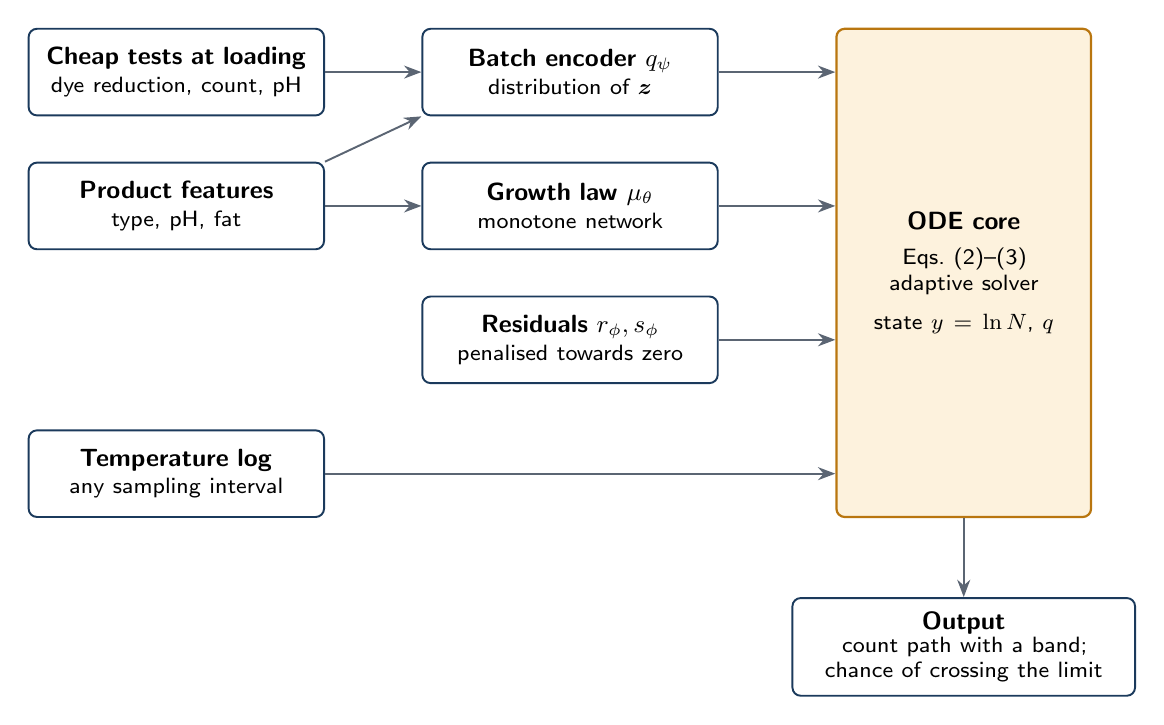
\begin{tikzpicture}[font=\sffamily\small,
  box/.style={draw=dgblue,line width=0.7pt,rounded corners=3pt,align=center,inner sep=5pt,text width=34mm,minimum height=11mm},
  arr/.style={-{Stealth[length=2.2mm]},draw=dggrey,line width=0.7pt}]
\node[box] (m) at (0,0) {\textbf{Cheap tests at loading}\\[-1pt]\footnotesize dye reduction, count, pH};
\node[box] (p) at (0,-1.7) {\textbf{Product features}\\[-1pt]\footnotesize type, pH, fat};
\node[box] (T) at (0,-5.1) {\textbf{Temperature log}\\[-1pt]\footnotesize any sampling interval};
\node[box] (enc) at (5,0) {\textbf{Batch encoder} $q_\psi$\\[-1pt]\footnotesize distribution of $\bm z$};
\node[box] (mu) at (5,-1.7) {\textbf{Growth law} $\mu_\theta$\\[-1pt]\footnotesize monotone network};
\node[box] (res) at (5,-3.4) {\textbf{Residuals} $r_\phi,s_\phi$\\[-1pt]\footnotesize penalised towards zero};
\node[draw=dgamberdk,fill=dgamber!18,line width=0.8pt,rounded corners=3pt,align=center,text width=30mm,minimum height=62mm] (ode) at (10,-2.55) {\textbf{ODE core}\\[3pt]\footnotesize Eqs.~(2)--(3)\\\footnotesize adaptive solver\\[3pt]\footnotesize state $y=\ln N$, $q$};
\node[box,text width=40mm] (out) at (10,-7.3) {\textbf{Output}\\[-1pt]\footnotesize count path with a band;\\[-2pt]\footnotesize chance of crossing the limit};
\draw[arr] (m)--(enc); \draw[arr] (p)--(mu); \draw[arr] (p.north east)--(enc.south west);
\draw[arr] (enc.east)--(enc.east-|ode.west); \draw[arr] (mu.east)--(mu.east-|ode.west); \draw[arr] (res.east)--(res.east-|ode.west);
\draw[arr] (T.east)--(T.east-|ode.west); \draw[arr] (ode)--(out);
\end{tikzpicture}
\caption{DairyGuard Neural. Known physics (the ODE core) is kept; networks learn the growth law, the departures from the textbook equations, and the hidden state of each batch}\label{fig:arch}
\end{figure}

\subsection{Observation model}
Plate counts are noisy. A measured count is modelled as $\log_{10}\hat N_k\sim\mathcal N\big(y(t_k)/\ln10,\ \sigma_{\mathrm{obs}}^2\big)$, with $\sigma_{\mathrm{obs}}$ learned and expected near 0.2 to 0.3 $\log_{10}$ units, and counts below the detection limit are treated as censored. When calorimetric data exist, the heat flow is modelled as $P=Y_QV\dd N/\dd t$, exactly as in DG-TR-01, which links heat-flow curves to the same state.

\subsection{Training}
The parameters $(\theta,\phi,\psi)$ are fitted by maximising the evidence lower bound,
\begin{equation}\label{eq:elbo}
\mathcal L=\sum_{\text{curves}}\Big(\mathbb E_{q_\psi(\bm z\mid\bm m)}\big[\log p(\hat N_{1:K}\mid\bm z,T)\big]-\mathrm{KL}\big(q_\psi(\bm z\mid\bm m)\,\|\,p(\bm z)\big)\Big)-\lambda\big(\|r_\phi\|^2+\|s_\phi\|^2\big),
\end{equation}
where the last term keeps the residuals small unless the data need them. The ODE is solved with an adaptive Runge--Kutta solver and differentiated through the solver or with the adjoint method \cite{chen2018}, using PyTorch and \texttt{torchdiffeq}. Training runs on a free Google Colab GPU; the model is small, tens of thousands of parameters, so a full training run is expected to take minutes to hours, not days.

\subsection{Uncertainty}
Two sources of uncertainty are kept apart: uncertainty about the batch, carried by the distribution of $\bm z$, and uncertainty about the model itself, estimated with a deep ensemble of five independently trained copies \cite{lakshminarayanan2017}. The probability of crossing the limit is the share of sampled paths that cross it, exactly as in the Monte Carlo monitor of DG-TR-01, and it is checked for calibration on held-out data.

\section{Three research questions}
The aim is not only a more accurate model. Each question below can produce a finding that is new whatever its answer.

\textbf{Q1. Does real milk run on one biological clock?} DG-TR-01 proves that, within the Baranyi--Roberts model, growth depends on temperature only through $\tau$. Whether real milk flora obey this is an experimental question. The size of the trained residuals $r_\phi$ and $s_\phi$, and the collapse or not of real curves when plotted against $\tau$, answer it. If they collapse, a single calorimetric or isothermal test can stand in for a whole temperature study. If they do not, the residuals show which kinds of temperature shift break the clock, for example a lag that reappears after a drop in temperature.

\textbf{Q2. Which cheap test buys the most accuracy?} The loss budget of DG-TR-01 prices information. With the encoder trained on real batches, the gain in AUC and in calibration from each test at loading (dye-reduction time, initial plate count, pH, a calorimetric detection time where available) can be measured and set against its cost. The result is a ranked list of what a dairy should measure, in rupees per unit of accuracy.

\textbf{Q3. Do chilled foods share a common hidden biology?} If the latent space $\bm z$ learned from milk transfers to other chilled products in ComBase (meat, fish, ready-to-eat foods) with little retraining, the hidden biology of cold-chain spoilage has a common structure. If it does not, the model shows which products need their own. Either answer decides whether one monitor can serve the whole cold chain.

\section{Data}
\subsection{Existing public data}
ComBase holds tens of thousands of growth records \cite{baranyi2004,combase}. DG-TR-01 used only maximum growth rates; DairyGuard Neural uses full growth curves: counts against time, including lag, for milk flora, \textit{Pseudomonas}, \textit{Listeria} and other organisms in chilled foods, and the records made under changing temperature. Published fluctuating-temperature studies that print their counts, such as Lin et al.\ \cite{lin2016}, are added. All of these are split by study, not by curve, so that a test set never shares a laboratory with the training set.

\subsection{New laboratory data}
Public data has two gaps that matter here: few curves of natural milk flora under realistic temperature shifts, and almost no curves paired with cheap measurements of the same batch. Four experiments close them (Table~\ref{tab:exp}). Counts follow the standard pour-plate method, ISO 4833-1 \cite{iso4833}, with psychrotrophic counts by ISO 17410 \cite{iso17410}.

\begin{table}[!htbp]\centering\footnotesize
\caption{Planned laboratory experiments}\label{tab:exp}
\begin{tabular}{@{}p{1.1cm}p{4.3cm}p{4.4cm}p{3.6cm}@{}}\toprule\rowcolor{dghead}
& What is done & Why & Answers\\\midrule
E1 & Pasteurised milk from 3 batches held at 4, 7, 10 and 15\degC; plate counts every 12 to 24\,h, in duplicate & Real growth curves of natural flora, with lag, to train $\mu_\theta$ on the actual product & Growth law; baseline for Q1\\
E2 & The same milk under steps up (4 to 12\degC), steps down (12 to 4\degC) and 4--12\degC{} cycles & Shifts are where the textbook equations are most likely to fail & Q1\\
E3 & At least 10 batches (brands and dates) under one realistic profile, with a dye-reduction test, an initial count and pH on day 0 & Batch-to-batch variation paired with cheap tests & Q2, encoder training\\
E4 & Isothermal microcalorimetry of the same batches, with a collaborating laboratory & Tests the calorimetric master curve and detection time on real milk & Q1, Q2\\
\bottomrule\end{tabular}\end{table}

E1 to E3 need about 300 to 400 plate counts and standard microbiology equipment: incubators or refrigerators held at set temperatures, an autoclave, a laminar-flow cabinet, plate count agar, pipettes and a colony counter. A microplate reader, if available, allows dye-reduction kinetics in many wells at once. The temperature steps and cycles of E2 can be run by a refrigerator under a simple microcontroller controller with a DS18B20 probe, which also logs the temperature. E4 needs an isothermal microcalorimeter, which is the reason to seek a partner laboratory.

\section{How it will be judged}
The rules below are fixed now, before any training.
\begin{itemize}
\item \textbf{Splits.} Training, validation and test sets are chosen by study and by batch before results are looked at. New laboratory batches used for testing are never used for training.
\item \textbf{Baselines.} DairyGuard Kinetic; a classical Baranyi--Roberts model with a fitted square-root law; and a pure black-box recurrent network of similar size. The hybrid has to beat the classical model to justify its networks, and has to beat the black box to justify its physics.
\item \textbf{Metrics.} Root-mean-square error of $\log_{10}$ counts; bias and accuracy factors \cite{ross1996}; AUC and expected calibration error for crossing the limit; coverage of the 90\,\% prediction band.
\item \textbf{Honesty.} Results on simulated data are labelled as simulation. A result that fails is reported as a failure.
\end{itemize}

\section{Timeline}
\begin{table}[!htbp]\centering\footnotesize
\caption{Plan to February 2027}\label{tab:time}
\begin{tabular}{@{}p{2.4cm}p{11.2cm}@{}}\toprule\rowcolor{dghead}
Month & Work and output\\\midrule
November 2026 & Data pipeline for ComBase growth curves. PyTorch and \texttt{torchdiffeq} prototype, first trained on curves simulated by DairyGuard Kinetic, where the right answer is known, to check that the code recovers it\\
December 2026 & Train the growth law $\mu_\theta$ on ComBase curves on Colab; compare with the square-root law. Approach laboratories for E1 to E4\\
January 2027 & Laboratory E1 and E2 begin; batch encoder trained on ComBase; residual networks switched on\\
February 2027 & First combined training on public and new data; held-out evaluation; model exported to the website demo; results written up as Technical Report DG-TR-02\\
After February & E3 and E4 complete; Q2 and Q3 answered in full; journal paper only once the laboratory results stand\\
\bottomrule\end{tabular}\end{table}

Laboratory data will be partial by February. The model is designed so that it can be trained on public data first and improved as each experiment finishes.

\section{From model to demo}
The trained model is exported as a small file of weights and run in the browser by the same demo that runs DairyGuard Kinetic today. Both models answer the same request, a temperature log plus any test results, with the same reply, a count path with a band and a probability of crossing the limit, so they can be compared side by side on the same trip.

\section{Risks}
\begin{itemize}
\item \textbf{Too little data for the encoder.} Ten batches may not be enough to learn $\bm z$. Fallback: a lower-dimensional $\bm z$ and stronger priors from ComBase.
\item \textbf{Laboratory access is delayed.} Fallback: complete the public-data parts of Q1 and Q3 first.
\item \textbf{Residuals absorb everything.} Fallback: a larger penalty $\lambda$, chosen on validation data, and a report of how the conclusions change with it.
\item \textbf{No calorimeter.} Q2 is then answered for the other tests only, and calorimetry stays a proposal.
\end{itemize}

\section*{Acknowledgements}
The author thanks the ComBase consortium and the laboratories whose published growth records make this work possible.

\section*{Note on tools}
The software for DairyGuard is written with the help of an AI coding assistant; every result is produced by tested code that the author has checked.

\begin{thebibliography}{99}\small\setlength{\itemsep}{1pt}
\bibitem{tr01} Singh SP. Beyond the 4\,\textdegree C alarm: what a temperature log can and cannot tell about milk spoilage. DairyGuard Technical Report DG-TR-01; 2026. \url{https://github.com/CopyNinja07-07/dairyguard}
\bibitem{baranyi2004} Baranyi J, Tamplin ML. ComBase: a common database on microbial responses to food environments. J Food Prot. 2004;67:1967--71. \url{https://doi.org/10.4315/0362-028X-67.9.1967}
\bibitem{combase} ComBase. Database of microbial responses to food environments. \url{https://www.combase.cc}
\bibitem{ratkowsky1982} Ratkowsky DA, Olley J, McMeekin TA, Ball A. Relationship between temperature and growth rate of bacterial cultures. J Bacteriol. 1982;149:1--5. \url{https://doi.org/10.1128/jb.149.1.1-5.1982}
\bibitem{baranyi1994} Baranyi J, Roberts TA. A dynamic approach to predicting bacterial growth in food. Int J Food Microbiol. 1994;23:277--94. \url{https://doi.org/10.1016/0168-1605(94)90157-0}
\bibitem{ozawa1986} Ozawa T. Non-isothermal kinetics and generalized time. Thermochim Acta. 1986;100:109--18. \url{https://doi.org/10.1016/0040-6031(86)87053-8}
\bibitem{malek2013} Málek J, Koga N, Pérez-Maqueda LA, Criado JM. The Ozawa's generalized time concept and YZ-master plots as a convenient tool for kinetic analysis of complex processes. J Therm Anal Calorim. 2013;113:1437--46. \url{https://doi.org/10.1007/s10973-013-2939-0}
\bibitem{lin2016} Lin H, Shavezipur M, Yousef A, Maleky F. Prediction of growth of \textit{Pseudomonas fluorescens} in milk during storage under fluctuating temperature. J Dairy Sci. 2016;99:1822--30. \url{https://doi.org/10.3168/jds.2015-10179}
\bibitem{ross1996} Ross T. Indices for performance evaluation of predictive models in food microbiology. J Appl Bacteriol. 1996;81:501--8. \url{https://doi.org/10.1111/j.1365-2672.1996.tb03539.x}
\bibitem{fricke2020} Fricke C, Harms H, Maskow T. How to speed up the detection of aerobic microbial contaminations by using isothermal microcalorimetry. J Therm Anal Calorim. 2020;142:1933--49. \url{https://doi.org/10.1007/s10973-020-09986-0}
\bibitem{rackauckas2020} Rackauckas C, Ma Y, Martensen J, Warner C, Zubov K, Supekar R, Skinner D, Ramadhan A, Edelman A. Universal differential equations for scientific machine learning. arXiv:2001.04385; 2020. \url{https://arxiv.org/abs/2001.04385}
\bibitem{sill1998} Sill J. Monotonic networks. In: Advances in Neural Information Processing Systems 10; 1998. p.~661--7.
\bibitem{kingma2014} Kingma DP, Welling M. Auto-encoding variational Bayes. International Conference on Learning Representations; 2014. \url{https://arxiv.org/abs/1312.6114}
\bibitem{rubanova2019} Rubanova Y, Chen RTQ, Duvenaud D. Latent ordinary differential equations for irregularly-sampled time series. In: Advances in Neural Information Processing Systems 32; 2019. \url{https://arxiv.org/abs/1907.03907}
\bibitem{chen2018} Chen RTQ, Rubanova Y, Bettencourt J, Duvenaud D. Neural ordinary differential equations. In: Advances in Neural Information Processing Systems 31; 2018. \url{https://arxiv.org/abs/1806.07366}
\bibitem{lakshminarayanan2017} Lakshminarayanan B, Pritzel A, Blundell C. Simple and scalable predictive uncertainty estimation using deep ensembles. In: Advances in Neural Information Processing Systems 30; 2017. \url{https://arxiv.org/abs/1612.01474}
\bibitem{iso4833} International Organization for Standardization. ISO 4833-1:2013 Microbiology of the food chain: horizontal method for the enumeration of microorganisms, part 1: colony count at 30\,\textdegree C by the pour plate technique. \url{https://www.iso.org/standard/53728.html}
\bibitem{iso17410} International Organization for Standardization. ISO 17410:2019 Microbiology of the food chain: horizontal method for the enumeration of psychrotrophic microorganisms. \url{https://www.iso.org/standard/67437.html}
\end{thebibliography}
\end{document}
